%!TEX root = ../main.tex
%%%%%%%%%%%%%%%%%%%%%%%%%%%%%%%%%%
% Links:
%
% Difficulty: Companies: 
%%%%%%%%%%%%%%%%%%%%%%%%%%%%%%%%%%


%\begin{figure} \centering 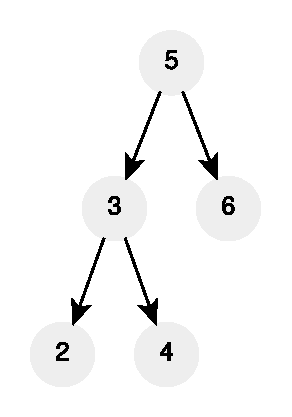
\includegraphics[width=\textwidth]{sources/decode_string/images/example1}
%   \caption[Sample short cpation]{Sample Caption}. \label{fig:decode_string:example1} \end{figure}

\chapter{Ways of decoding a message}
\label{ch:decode_string}
\section*{Introduction}
This problem resemble the problem of decoding a string encoded with the famous \textit{run-length
encoding method}(RLE)\footnote{It is a simple form of data compression in
which a stream of data is given (like the following string "AAABBCCCC") 
and the output is a sequence of	counts of consecutive data values in a row. 
(i.e. "3A2B4C").
It is a type of lossless encoding meaning that the encoding process does not lose any information in the 
original input and therefore the input data can be recovered fully and integrally.
decoded.} 

The problem discussed in this chapter is going to deal with a similar algorithm and you are asked to write a 
decode function for a string encoded with a run-length-encoding-like algorithm.


\section{Problem statement}
\begin{exercise}
\label{example:decode_string:exercice1}
Write a function that given an encoded string $s$ decodes it.
$s$ is of the form: ${k_1[d_1]k_2[d_2[ \ldots]}$ where $k$ is a positive integer and $s$ is another encoded string. 
The decoded version of $s$ is obtained by appending $d_1$ $k_1$ followed by repeating $d_2$ $k_2$ times.
 
	%example1
	\begin{example}
		\label{example:decode_string:example1}
		\hfill \\
		Given \inline{s="2[abc]3[ab]"} the function returns \inline{"abcababababcababab"}.
	\end{example}

	%example2
	\begin{example}
		\label{example:decode_string:example2}
		\hfill \\
		Given \inline{s="2[abc3[ab]]"} the function returns \inline{"abcababababcababab"}.
	\end{example}

	\begin{example}
		\hfill \\
		Given \inline{s="2[abc]3[cd]ef"} the function returns \inline{"abcabccdcdcdef"}.

	\label{ex:decode_string:example3}
	\end{example}
\end{exercise}

\section{Clarification Questions}

\begin{QandA}
	\item Is it guaranteed that $s$ is always valid?
	\begin{answered}
		\textit{Yes, $s$ contains only lower-case letters from the English alphabet, numbers and square brackets and it is valid encoded string. .}
	\end{answered}

\end{QandA}

\section{Discussion}
\label{decode_string:sec:discussion}


\subsection{Recursive solution}
\label{decode_string:sec:recursive}
The first thing we notice about this problem is that the encoded string has a recursive definition. 
Whenever we encounter a number $x$ followed by the \inline{'['} character we are know that we have to 
decode whatever is inside the square brackets and then repeat that $x$ times. 
We can use this fact to simply create a recursive algorithm which mimics this definition. The real challenge of this problem
lies in the implementation more than in the algorithm itself.

The idea is to construct the final answer by looking at one character of $s$ at a time. 
We can start from char at index $0$ and depending from it we can:
\begin{enumerate}
	\item append it to the answer (when the char we are looking at is a letter)
	\item parse it as a part of a number (when we encounter a digit) or,
	\item recursively decode the rest of the string (when the current character is an open square bracket \inline{'['}).
\end{enumerate}.
For instance image we have to decode \inline{s="xy242[ab3[c]de]}. 
We start by reading $x$ and $y$ which are letters and therefore are just appended to the final answer.
We then see a digit, which signal us that a number started.  We parse it fully into the number $242$.The end of the number is signaled by the presence of the char \inline{'['}
which also signals that a new encoded substring is starting. 
So when we see an open square bracket character we recursively call the decode function so that it returns the expansion of whatever is within the brackets. 
When the recursive call ends (when we find a closed square bracket character \inline{']'})
 we are left with the expanded string which we can then replicate $242$ times and append to the final answer. 
Each recursive function also update the index which signals the next character in the input string that is not yet processed. 
This is necessary because after the recursive call we might need to continue processing more characters.
Listing \ref{list:decode_string:recursive} shows a possible implementation of this idea.
Notice that the function \inline{decode_string_recursive_helper} takes as a second parameter a reference to an index of $i$.
We use a reference because we want this number to be updated by each of the recursive calls.
We use $i$ to keep track of the current character we are examining in $s$.


\lstinputlisting[language=c++, caption={Sample Caption},label=list:decode_string:recursive]{sources/decode_string/decode_string_solution2.cpp}


\begin{figure}
	\centering
	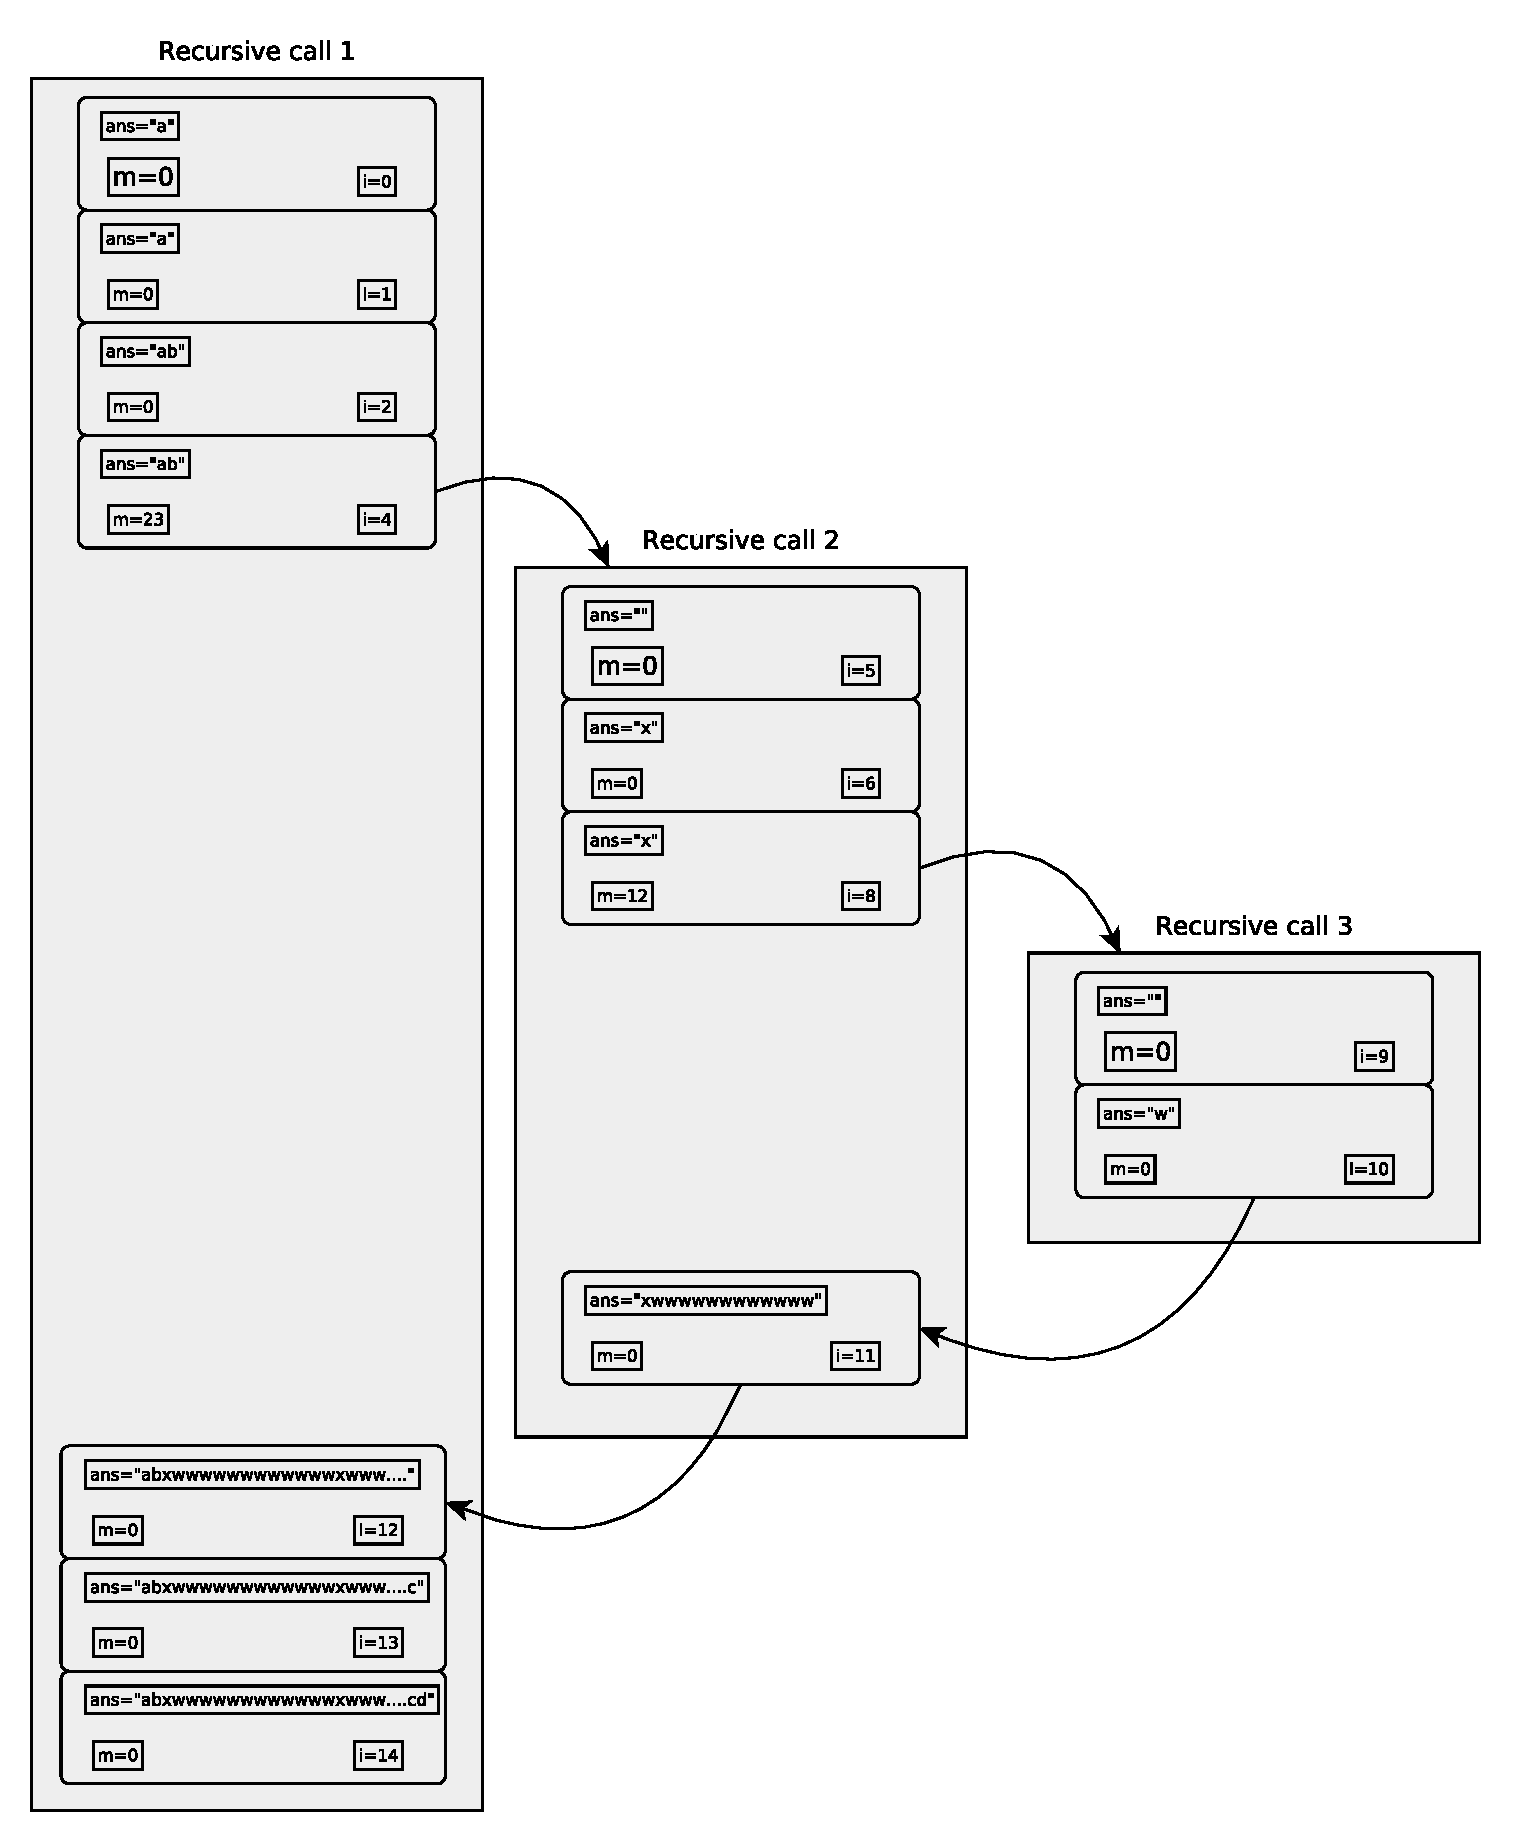
\includegraphics[width=\textwidth]{sources/decode_string/images/recursion}
   \caption{Execution of the algorithm in Listing \ref{} for the input string \inline{s="ab23[x12[w]]cd}}. \label{fig:decode_string:recursion}
 \end{figure}



\lstinputlisting[language=c++, caption={Sample Caption},label=list:decode_string]{sources/decode_string/decode_string_solution2.cpp}
